\documentclass[12pt,leqno]{amsart}
\usepackage{pgfplots}       % it also load tikz package
\pgfplotsset{compat=1.17}   
\usetikzlibrary{arrows.meta}
\usepackage{tikz}
\usepackage{tcolorbox}
\usetikzlibrary{shapes.geometric, arrows, snakes, backgrounds}
\tikzstyle{startstop} = [rectangle, rounded corners, minimum width=3cm, minimum height=1cm,text centered, draw=black, fill=red!30]
\tikzstyle{io} = [trapezium, trapezium left angle=70, trapezium right angle=110, minimum width=1cm, minimum height=1cm, text centered, draw=black, fill=blue!30]
\tikzstyle{process} = [rectangle, minimum width=1cm, minimum height=1cm, text centered, draw=black, fill=orange!30]
\tikzstyle{decision} = [diamond, minimum width=1cm, minimum height=1cm, text centered, draw=black, fill=green!30]
\tikzstyle{arrow} = [thick,->,>=stealth]
\usepackage{tcolorbox}
\usepackage{caption}
\usepackage[colorlinks=true,
            citecolor={black}]{hyperref}
\usepackage{lipsum} % added for generating a dummy text, 
                    % not needed in real document
\usepackage{fancyvrb}
\begin{document}
%\lipsum[1]  % dummy text
%\begin{tcolorbox}[colback=white]
\begin{comment}


\newpage
\paragraph{\textbf{1.NER regex}}
It contains the main script "ner\_regex.py" and the "Dataset" folder.
The Dataset folder is provided with an example "soa.csv" input file containing documents.
\paragraph{\textbf{Usage:}}
The user can just execute the script ner\_regex.py.
This module is meant to find text-instances of SOA data and to label them.
\paragraph{\textbf{Output:}}
a .json1 file containing annotations that describe the retrieved entities.

\end{comment}
\tikzstyle{place}=[circle,draw=blue!50,fill=blue!20,thick]
\tikzstyle{transition}=[rectangle,draw=black!50,fill=black!20,thick]
\begin{tikzpicture}
\node[place] (waiting) {};
\node[place] (critical) [below of=waiting] {};
\node[place] (semaphore) [below of=critical] {};
\node[transition] (leave critical) [right of=critical] {};
\node[transition] (enter critical) [left of=critical] {};
\node [red,above] at (semaphore.north) {$s\le 3$};
\begin{pgfonlayer}{background}
\filldraw [fill=black!30,draw=red] (0,0) rectangle (2,1);

\end{pgfonlayer}
\end{tikzpicture}
			
%\filldraw [fill=black!30,draw=red] (semaphore.south -| enter critical.west) rectangle (waiting.north -| leave critical.east);
%REGEX NER
	\begin{figure}[ht] % placed here or on the top of page
		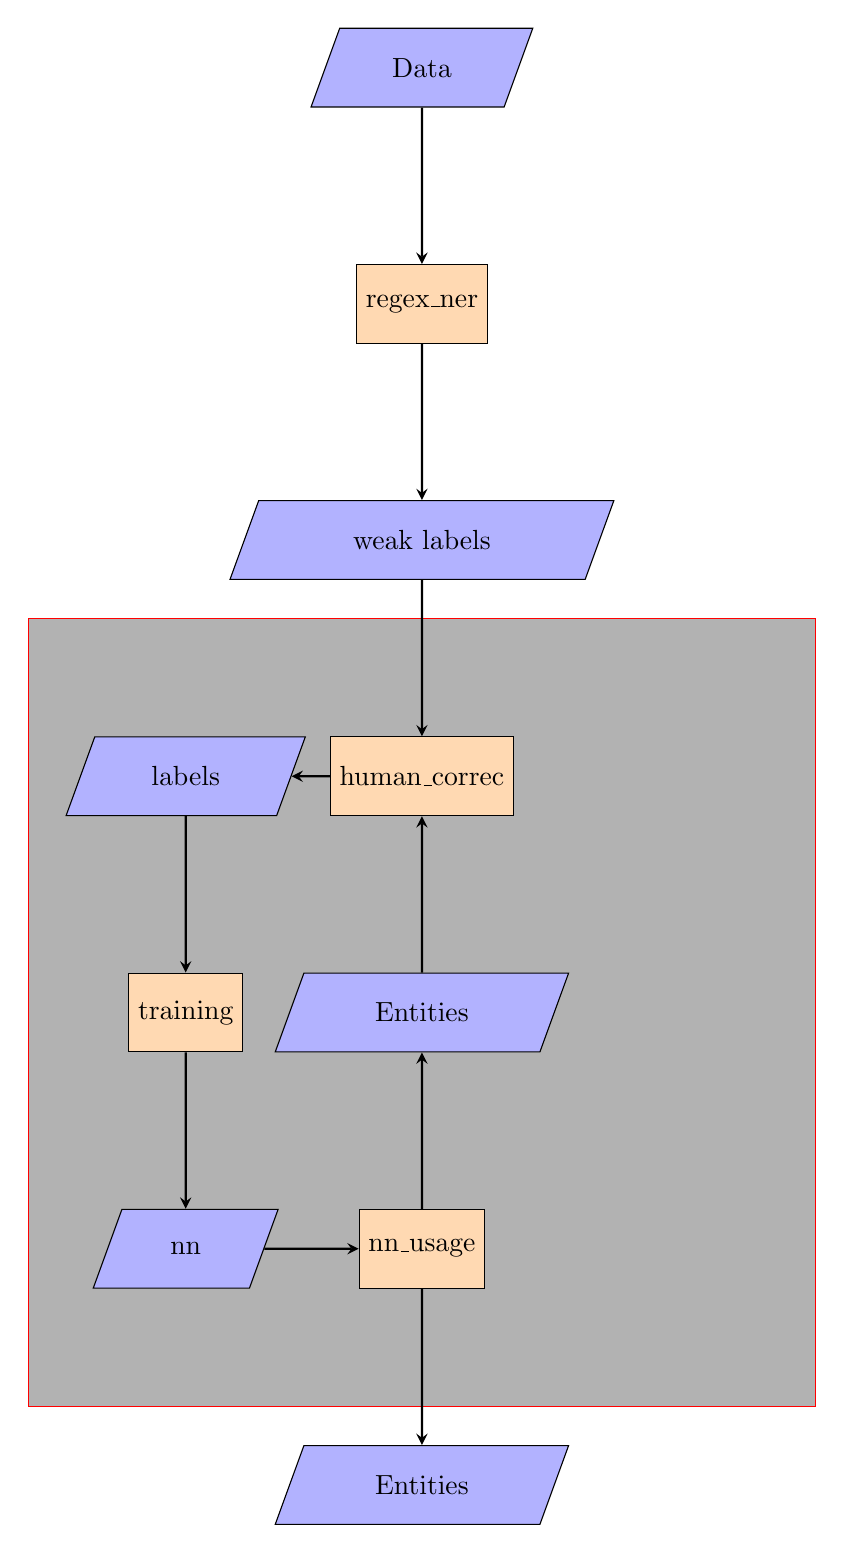
\begin{tikzpicture}[node distance=3cm]
		%\begin{tikzpicture}%[->,shorten >=1pt,auto,node distance=2.8cm,semithick]
			\node (data) [io] {Data};
			\node (module0) [process, below of=data] {regex\_ner};
			\draw [arrow] (data) -- (module0);
			\node (wl) 		[io, below of=module0] {weak labels};
			\draw [arrow] (module0) -- (wl);
			\node (humcorr) [process, below of=wl] {human\_correc};
			\draw [arrow] (wl) -- (humcorr);
			\node (l) 		[io, left of=humcorr] {labels};
			\draw [arrow] (humcorr) -- (l);
			\node (train) 	[process, below of=l] {training};
			\draw [arrow] (l) -- (train);
			\node (nn) 		[io, below of=train] {nn};
			\draw [arrow] (train) -- (nn);
			\node (module) [process, right of=nn] {nn\_usage};
			\draw [arrow] (nn) -- (module);
			\node (entities) [io, below of=module] {Entities};
			\node (entitiescorr) [io, above of=module] {Entities};
			\draw [arrow] (module) -- (entities);
			\draw [arrow] (module) -- (entitiescorr);
			\draw [arrow] (entitiescorr) -- (humcorr);
			
\begin{pgfonlayer}{background}
\filldraw [fill=black!30,draw=red] (5,-7) rectangle (-5,-17);
%\filldraw [fill=black!30,draw=red] (nn.south -| nn.west) rectangle (humcorr.north -| entitiescorr.east);
\end{pgfonlayer}
		\end{tikzpicture}
		\caption{Human In The Loop framework} % caption
		%\label{fig:diagram}             % for referencing of figure, key select as you wish
	\end{figure}
%\lipsum[2]  % dummy textù


\end{document}